\chapter{Эксперименты}
\label{chap:experiments}

\section{Тестовая выборка}
Для тестирования разработанной схемы для создания классификаторов необходимо создать тестовую выборку. Данная глава описывает четыре набора данных использованных для тестирования.

\subsection{Тематические классы}
Данный тестовый набор состоит из следующих классов:
\begin{itemize}
\item Физика
\item Химия
\item Биология
\item Математика
\item Программирование
\end{itemize}

Для каждого из классов были выбраны несколько пользователей ``Твиттера'', которые пишут на данную тему. Они перечислены в Таблице \ref{table:thematic}. Далее для каждого из пользователей в выборку вошли случайные 100 записей из последних 2000.

В качестве способа тестирования было выбрано два варианта: перекрёстная проверка с разделением на 4 части и тестовая выборка составленная из записей пользователей отличных от тех, что использовались в обучающей выборке.

\subsection{Целевые классы}

Данный тестовый набор частично взят из работы \cite{Horn_2010}. Он состоит из классов:
\begin{itemize}
\item Новостных сообщений
\item Персональных сообщений
\item Сообщений из официальных ``Твиттер'' аккаунтов компаний
\end{itemize}

Как и предыдущий, этот тестовый набор составлялся на основе пользователей ``Твиттера''. В Таблице \ref{table:unc} перечислены пользователи с классами к которым они были отнесены.

В качестве способа тестирования была выбрана перекрёстная проверка с разделением на 4 части и тестовая выборка составленная из записей пользователей отличных от тех, что использовались в обучающей выборке.

\section{Алгоритмы}
\subsection{Простая классификация}
К данной секции относятся следующие классифицирующие алгоритмы: \begin{itemize}
\item наивный байесовский,
\item метод опорных векторов,
\item метод J48 для построения деревьев принятия решений.
\end{itemize}

Все эти алгоритмы на вход принимают объекты из пространства признаков, так что использовалось два метода для выделения признаков из текста: \begin{itemize}
\item простая модель, описанная в секции \ref{sec:text-model};
\item модель на основе ``Википедии'' (далее --- энциклопедическая), описанная в секции \ref{sec:wiki-model}.
\end{itemize}

В общем получается 6 вариантов алгоритма.

\subsection{Классификация с учетом контекста}
В данной секции использовался предложенный в работе алгоритм классификации. В качестве базового алгоритма были использованы те же алгоритмы, что и в предыдущей секции, аналогично для алгоритма выделения признаков из текста. В качестве кластеризующих были использованы следующие алгоритмы: \begin{itemize}
\item k-means на 20 кластеров,
\item k-means на 100 кластеров,
\item xmeans с параметрами от 20 до 100 кластеров.
\end{itemize}

Во всех алгоритмах в качестве метрики для расстояния использовалась евклидова метрика\footnote{http://ru.wikipedia.org/wiki/Евклидова\_метрика}. Количество последних сообщений для кластеризации --- 2000.

В общем получается 18 вариантов алгоритма.

\section{Результаты экспериментов}

% Тематические классы: тестовая выборка
\begin{figure}[h!]
  \centering
    \includegraphics[width=\textwidth]{thematic/test/naive}
    \caption{Тематические классы: тестовая выборка; наивный байесовский классификатор}
    \label{fig:thematic-test-naive}
\end{figure}

\begin{figure}[h!]
  \centering
    \includegraphics[width=\textwidth]{thematic/test/svm}
    \caption{Тематические классы: тестовая выборка; метод опорных векторов}
    \label{fig:thematic-test-svm}
\end{figure}

\begin{figure}[h!]
  \centering
    \includegraphics[width=\textwidth]{thematic/test/j48}
    \caption{Тематические классы: тестовая выборка; алгоритм построения деревьев решений J48}
    \label{fig:thematic-test-j48}
\end{figure}

% Тематические классы: перекрёстная проверка
\begin{figure}[h!]
  \centering
    \includegraphics[width=\textwidth]{thematic/cross/naive}
    \caption{Тематические классы: перекрёстная проверка; наивный байесовский классификатор}
    \label{fig:thematic-cross-naive}
\end{figure}

\begin{figure}[h!]
  \centering
    \includegraphics[width=\textwidth]{thematic/cross/svm}
    \caption{Тематические классы: перекрёстная проверка; метод опорных векторов}
    \label{fig:thematic-cross-svm}
\end{figure}

\begin{figure}[h!]
  \centering
    \includegraphics[width=\textwidth]{thematic/cross/j48}
    \caption{Тематические классы: перекрёстная проверка; алгоритм построения деревьев решений J48}
    \label{fig:thematic-cross-j48}
\end{figure}

% Целевые классы: тестовая выборка
\begin{figure}[h!]
  \centering
    \includegraphics[width=\textwidth]{usernewscompany/test/naive}
    \caption{Целевые классы: тестовая выборка; наивный байесовский классификатор}
    \label{fig:usernewscompany-test-naive}
\end{figure}

\begin{figure}[h!]
  \centering
    \includegraphics[width=\textwidth]{usernewscompany/test/svm}
    \caption{Целевые классы: тестовая выборка; метод опорных векторов}
    \label{fig:usernewscompany-test-svm}
\end{figure}

\begin{figure}[h!]
  \centering
    \includegraphics[width=\textwidth]{usernewscompany/test/j48}
    \caption{Целевые классы: тестовая выборка; алгоритм построения деревьев решений J48}
    \label{fig:usernewscompany-test-j48}
\end{figure}

% Целевые классы: перекрёстная проверка
\begin{figure}[h!]
  \centering
    \includegraphics[width=\textwidth]{usernewscompany/cross/naive}
    \caption{Целевые классы: перекрёстная проверка; наивный байесовский классификатор}
    \label{fig:usernewscompany-cross-naive}
\end{figure}

\begin{figure}[h!]
  \centering
    \includegraphics[width=\textwidth]{usernewscompany/cross/svm}
    \caption{Целевые классы: перекрёстная проверка; метод опорных векторов}
    \label{fig:usernewscompany-cross-svm}
\end{figure}

\begin{figure}[h!]
  \centering
    \includegraphics[width=\textwidth]{usernewscompany/cross/j48}
    \caption{Целевые классы: перекрёстная проверка; алгоритм построения деревьев решений J48}
    \label{fig:usernewscompany-cross-j48}
\end{figure}

Для начала хотелось бы отметить, что метод опорных векторов продемонстрировал наилучшие результаты на наших тестовых данных (рисунки  \ref{fig:thematic-test-svm}, \ref{fig:thematic-cross-svm}, \ref{fig:usernewscompany-test-svm}, \ref{fig:usernewscompany-cross-svm}). Кроме того, метод опорных векторов больше всех выигрывает от использования контекста в классификаторе (это лучше заметно на рисунках соответствующих тематической тестовой выборке: \ref{fig:thematic-test-svm} и \ref{fig:thematic-cross-svm}). Меньше всех выигрывает, а иногда даже проигрывает от использования контекста наивный байесовский классификатор. Также можно видеть не самый успешный результат алгоритма J48 в случае использования простой модели текста (Рис. \ref{fig:thematic-cross-j48}).

При использовании энциклопедической модели теста, к сожалению, результат простых классификаторов значительно ухудшился. Этот результат показывает, что данный аспект, по всей видимости, нуждается в улучшении. Однако стоит отметить, что использование контекста в случае энциклопедической модели позволяет получить значительное (порядка 20\% на Рис. \ref{fig:thematic-test-svm}) улучшение показателей классификатора. Связка признаков из ``Википедии'', использования контекста и метода опорных векторов продемонстрировала наилучший результат в данной работе.

Стоит отметить, что при использовании контекста, улучшение на первом наборе данных было больше чем на втором. Это выглядит разумным в свете того, что кластеризация более вероятно объединяет сообщения похожие тематически, чем по каким-либо других критериям. 

Из алгоритмов кластеризации наиболее предпочтительно выглядит XMeans. Именно этот алгоритм рекомендуется использовать при использовании контекстной классификации.